\documentclass[12pt,twocolumn]{article}
\usepackage[margin=0.7in]{geometry}
\usepackage{graphicx}
\usepackage{cite}
\linespread{1.5}
                                        
%%%%%%%%%%%%%%%%%%%%%%%%%%%%%%%%%%%%%%%%%%%%%%%%%%%%%%%%%%%%%%%%%%%%%%%%%%%%%%%%%%%%%%%%%%%%%%%%%%%%%%%%%%%%%%%%%%%%%%%%%%%%%%%%%%%%%%%%%%%%%%%%%%%%%%%%%%%%%%%%%%%%%%%%%%%%%%%%%%%%%%%%%%%%%%%%%%%%%%%%
                                        
\begin{document}
\title{A Muon's lifetime}
\author{M. Lane and Joseph Hartsell}
\date{\today}

\maketitle


\begin{abstract}
Using a Teach Spin Scintillator, mean muon lifetime was measured by histogram decay half-time measurements in this experiment. The muon proper lifetime was determined to be 2.19 $\mu$s. The rate of measured muon flux was compared with known values to verify relativistic time-dilation effects and we examined briefly the Fermi Constant.
\end{abstract}

\section{Introduction}
 Muons are a negatively charged lepton similar to the electron except with 200 times the mass. It is most frequently found in cosmic radiation.  The first time the muon decay was measure was in 1941 when  F. Rasetti showed that muon’s have a finite ”lifetime” now known to be 2.19 μs \cite{COSBUL}. Today thanks to the particle data group we know the value to actually be 2.196981 ± 0.000002 μs \cite{PDG}  (for some reason the citation software is not working properly). The muon, along with its positively charged counterpart the antimuon are the make up the second lepton group.  Their mean production altitude is 15km above sealevel \cite{PDG} and assuming they travel normal to Earth's surface we expect the travel time to reach earth is then: $15km/c = 50\mu s$. Much larger than their mean lifetime. Muons are often the decay product of negative pions that decay them selves from decay of free protons in the atmosphere. Figure below is has sketch of these primary decays of cosmic ray radiation, which naturally occurs in Earth’s upper atmosphere due to primary cosmic rays interactions with air molecules. Cosmic rays include protons, neutrons, pions, kaons, delta-ons, Helium, and other particles from the air is not understood well \cite{COSBUL}; suffices to know that pions are released which spontaneously decay into a muon and neutrino via the processes below \cite{COSBUL} and as shown on the figure:
\begin{figure}[h!]
	\centering
	\label{fig:Cosmic}
	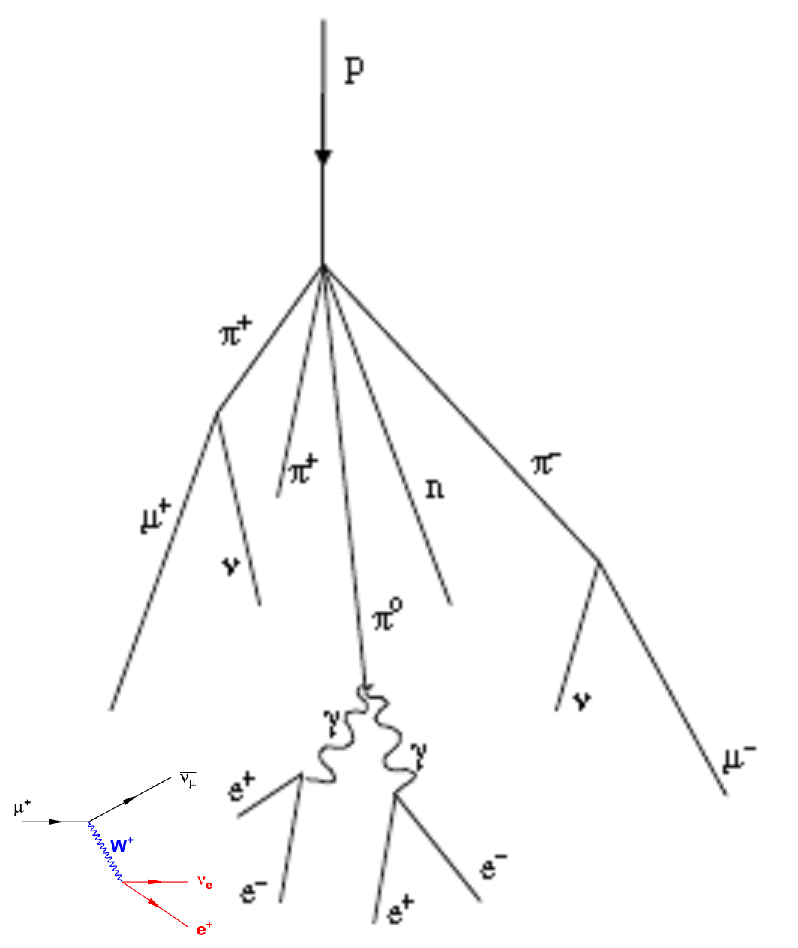
\includegraphics[width=3in]{images/Cosmic}
	\caption{Labratory Setup showing the scintillator and other devices}
\end{figure}
In turn muons naturally decay is:
\begin{equation}
	\label{eq:PionDecay}
	\begin{array}{c}
	\pi^{-} \rightarrow\mu^{-}\bar{\nu}_{\mu} \\
    \pi^{-} \rightarrow\mu^{-}\bar{\nu}_{\mu} \\
\end{array}
\end{equation}
As shown by Fermi diagram, this decay is mediated by the W boson. In fact, the fundamental constant of interaction of the weak electric force, called the Fermi constant $G_Fermi$, is best measured using the muon half-life and they are related by the following equation:
\begin{equation}
	\label{eq:Gf}
	\Rightarrow \frac{G_F}{(\hbar c)^3}=\sqrt{\frac{\hbar}{\tau_\mu}\cdot\frac{19 2\pi^3}{(m_\mu c^2)^5}}
\end{equation}

Relativistically, the muons produced travel at speeds near 99 percent the speed of light \cite{PDG}; however, our detector only detects those that are going .8c \cite{MUON}.  Due to the vast number of muons have been detected on Earth's surface shows that they cannot have a mean lifetime of $~2\mu s$ and travel time of $50\mu s$, as calculated from the the non relativistic speed. This is due o this as evidence for time dilation. Instead muons experience a time dilation of $t'=t_{0}/\gamma$, with $\gamma=\left(1-\beta^{2}\right)^{-1}$. With the velocity given above, we then expect the particles to experience a travel time 500 times less than previously predicted. We also include for the velocity decrease as the muon travels through air medium. The energy loss for a muon \cite{MUON} is:

\begin{equation}
	\label{eq:decaytime}
	\Delta E = 2 MeV/g/cm^{2} \cdot H \cdot \rho
\end{equation}

Where $\rho$ is the fluid density and $H$ is the height traveled through. We then note that
$dE=\rho C_{0} dh$, and from Einstein's relation we have $E=\gamma mc^{2}, dE=mc^{2}d\gamma$
which gives:

\begin{equation}
	dh = \frac{mc^{2}}{\rho C_{0}} d\gamma
\end{equation}

Noting that the travel time in the particle's rest frame is given by $dt'=dh / \left( c\beta\gamma \right)$
then gives:

\begin{equation}
	t' = \frac{mc}{\rho C_{0}} \int_{\gamma_{1}}^{\gamma_{2}} \frac{ d\gamma }{ \beta\gamma } = \frac{mc}{\rho C_{0}} \int_{\gamma_{1}}^{\gamma_{2}} \frac{ d\gamma }{ \sqrt{ \gamma^{2}-1 } }
\end{equation}


\begin{equation}
	t' = \frac{mc}{\rho C_{0}} \left.\log\left(\sqrt{\gamma^{2}-1}+\gamma\right)\right|_{\gamma_{1}}^{\gamma_{2}}
\end{equation}

Thus, muons reach the Earth's surface with a kinetic enery near 4GeV corresponding to $\gamma_{1}=38$. Using $\Delta E$ from Eq. \ref{eq:decaytime}, Therefore, the the upper atmosphere to be $\gamma_{2}=54.$ Using these values as the integral bounds gives a reasonable $t'=1.18\mu s$ in agreement with  the first order calculation.  A table of these calculations are give in the table at the end of this report.
 Given hat muons decay at a constant rate in any medium, we have $dN=\lambda dt$. This gives the familiar
 equation, we shall use to find the muon life time:
 \begin{equation}
	 \label{eq:probability}
	 N=N_{0}exp(-\lambda t)
 \end{equation}
 
 Where $\lambda$ is used to define the mean lifetime as $\lambda=1/\tau$.  This can 
 now be used to determine a height difference necessary for an experiment. Suppose we wished to measure and
 compare muon counts at two different elevations. Use For a noticeable difference between the two locations, we will say
 the time difference for the muon between the two locations should be $t'\approx 0.16\cdot\tau$ which gives $1-e^{-0.1}\approx10\%$ difference in muon counts between the two locations.

By using $t'=0.16\tau$ we find $\Delta\gamma\approx15=\Delta E / mc^2$. Which is nearly the same change experienced from the height of the atmosphere to sea-level. To truly perform a elevation varying experiment, very sensitive equipment should be used and a difference in muon counts less than 1\% must be able to be accurately measured.

In this experiment, we will use Eq. \ref{eq:probability} to measure the mean proper lifetime of muons. First note that the probability distribution is exponential, a memoryless probability distribution. This means the muons we may detect in the laboratory will decay under the same distribution despite having already traveled through the atmosphere. By fitting an exponential to measured decay times, we may measure the proper mean lifetime.

\section{Method}

In order to detect muon decays, we will utilize a plastic scintillator. When a charged particle enters the scintillator it will begin to slow, emitting light as it looses energy. A photodetector then begins a timer when a flash indicates a particle has entered. If a muon enters with sufficiently low kinetic energy, it will stop inside the scintillator and decay. When it decays, it emits photons which tells the photodetector to stop the timer. In this way, the time needed for a muon to decay is measured. If no secondary flash is detected within a brief period, the particle is assumed to have passed through without decaying, or is not a muon and not recorded as an event.

\begin{figure}[h!]
	\centering
	\label{fig:scin}
	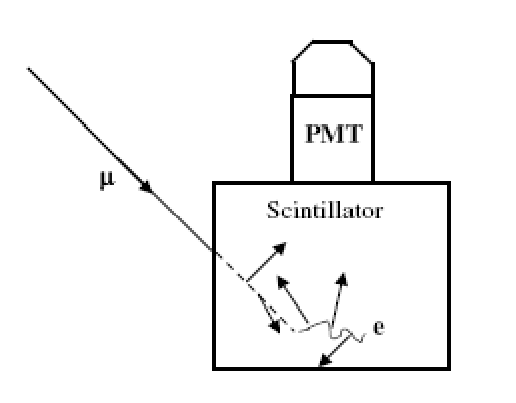
\includegraphics[width=3in]{images/scintillatorevents}
	\caption{Photon emission used in determining the lifetime of a muon}
\end{figure}
\begin{figure}[h!]
	\centering
	\label{fig:scin2}
	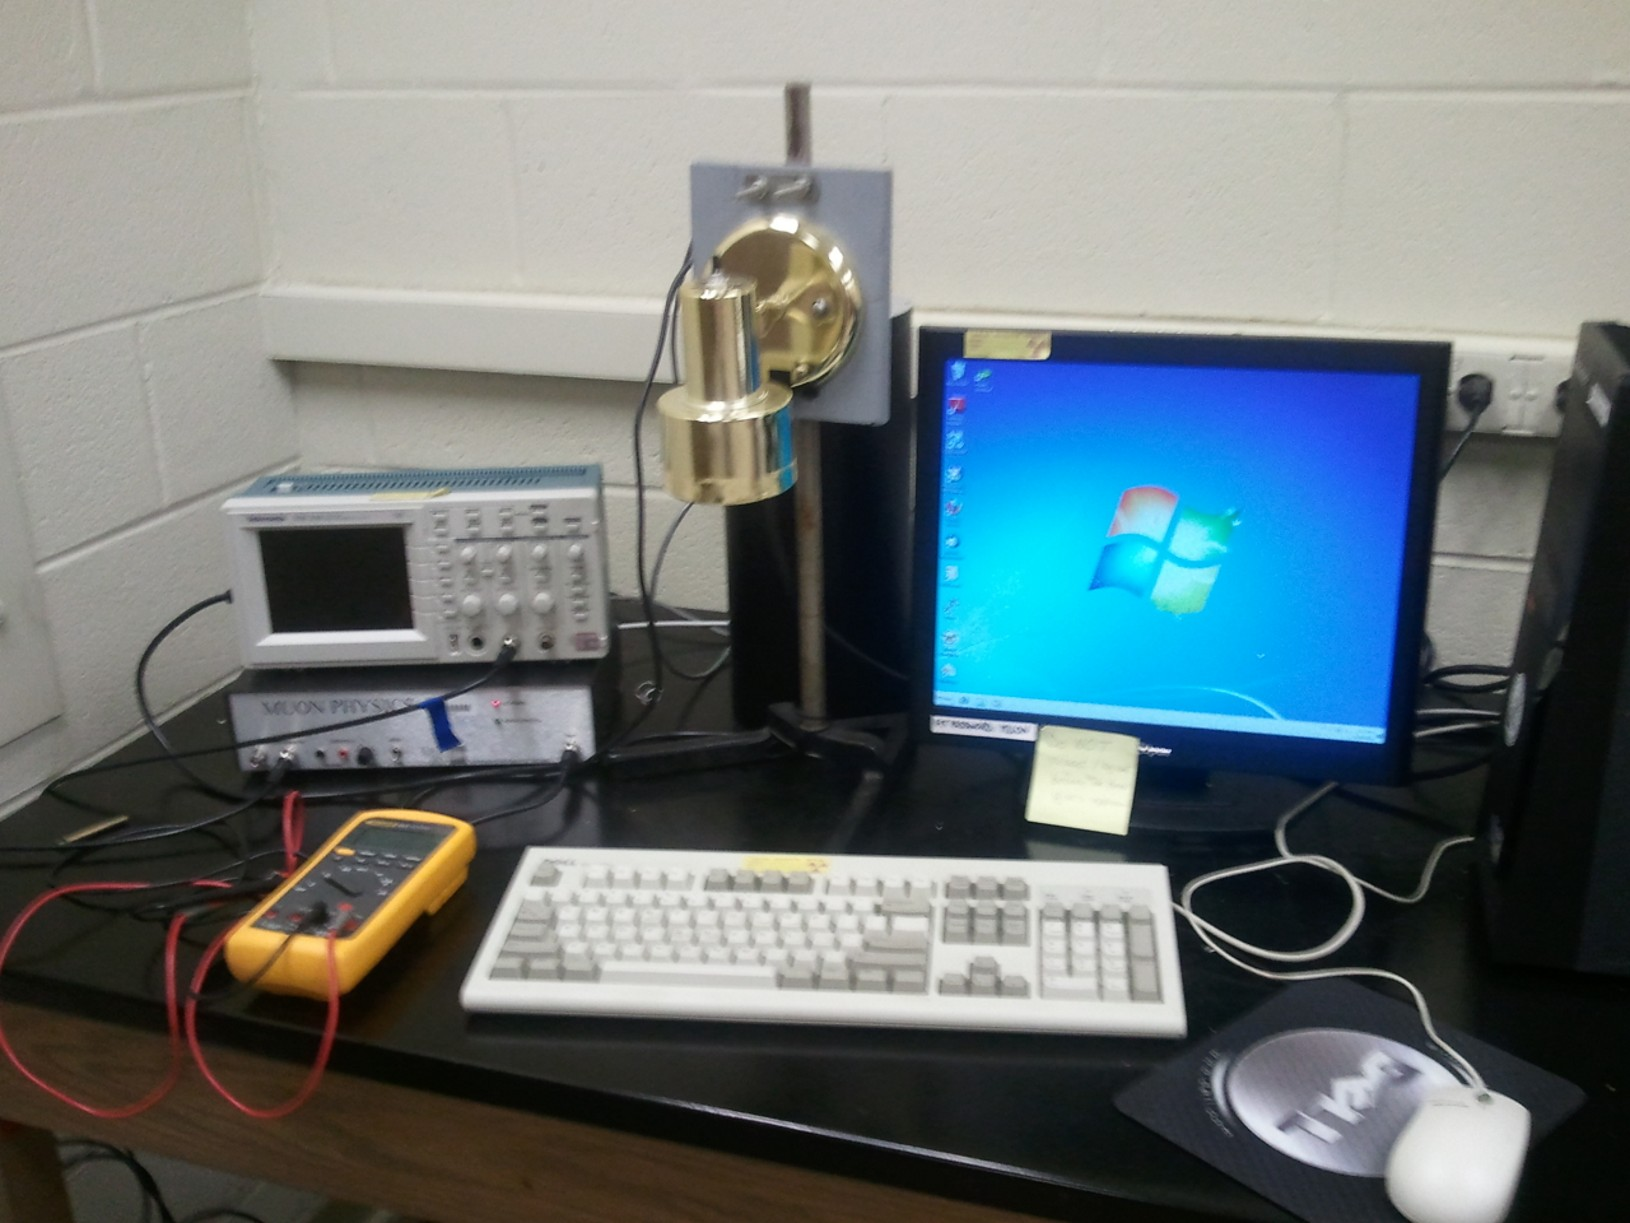
\includegraphics[width=3in]{images/Photo}
	\caption{Labratory Setup showing the scintillator and other devices}
\end{figure}

We recorded data from  3:00pm on June 5th, 2012 to  6:00pm June 19th, 2012.  The figure above shows the labratory setup with the black box being the scintillator.  The scintillator was connected to a computer which recorded the time of each event, and the time (in nanoseconds) between the initial flash and decay flash of a given event.  Inside the scintillator is a photomultiplier tube, or detector that converts photon emitted either by muon decay or electron collisions, into electrons and where the electrons are captured in current then transformed into a digital signal. A Photomultipler Tube consists of a photocathode and several diodes in a vacuum.  Typically, photomultipler tubes are build with whatever collaminator or attenuator already attached to \cite{PDG} .  In the PMT there is a special photocathode that converts photons to electrons, or ““photoelectrons””, via the photoelectric effect.  Through, using the secondary emission effect these electrons hit the various diodes increasing the current of going through the device.  In modern day times, this current is then translated, via a chip into a digital signal that is readable by a computer.  The formulas for time of flight and example of how they could detect are added.  As one may notice the time of flight depends on the Lorentz factor γ (and thus the velocity) of the original particle by an inverse relationship as expected.  Recall that as the original particle, in our case the muon, gets higher and higher Energy it moves faster due to  $E=γmc^2→E_light=mc^2$  witch $γ →1$.  Due γ=1 parts of formula for time of flight are basically washed out, therefore photomultiplier tubes cannot really detect high-energy particles, very well and differentiate between muons and electrons. Additionally most of the time the light need to be collaminated or attenuated for a photomultiplier tube to work properly.

\section{Analysis}

In the experiment we only actually measured the time between entering and decaying in nanoseconds and the time of the measurement.  These results were plotted on a histogram and then used . The initial histogram is shown below.

\begin{figure}[h!]
	\centering
	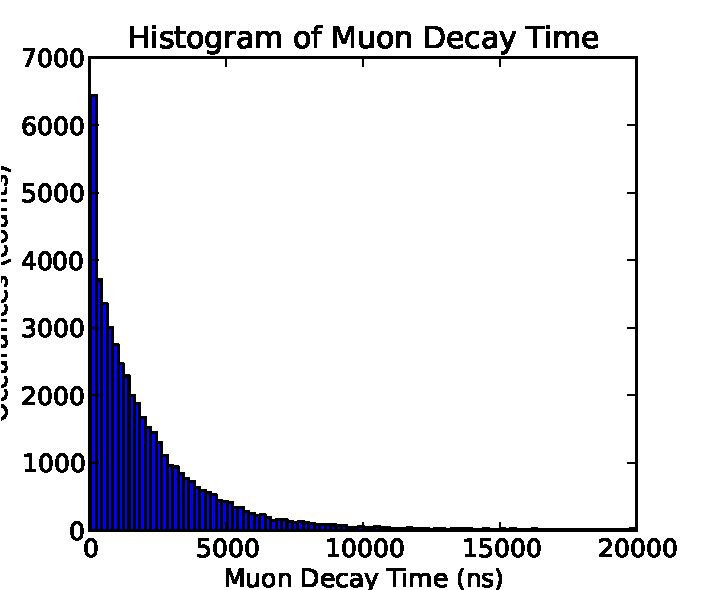
\includegraphics[width=3in]{images/Histogram-eps-converted-to}
	\caption{Raw Histogram}
	\label{fig:Histogram}
\end{figure}

With some foresight that the proper lifetime is near $2\mu s$, we mas safely assume that counts above $10\mu s$ are
noise and interference and should not be included in the analysis. Therefore, to calculate proper lifetime, we take
the logarithm of Eq. \ref{eq:probability} to obtain:

 \begin{equation}
	 \label{eq:probability}
	 \log(N)=\frac{-t}{\tau} + \log(N_{0})
 \end{equation}

 We fit the data on a semilog plot where The slope of the line gives the decay rate.  In order to get an accurate value the background noise is then subtracted out and the fit calculation redone. Using this method we found the slope of the fit line to be -0.4550 indicating $\tau=2.19 +/- .01$ in agreement with known values /cite{PDG}.  We compared this to separate trials of the muon data for each run we did (see appendix). At fist glance, the results imply that the lifetime would be more accurate the more time we allow the detector to run. however, trail 2 and 4 suggestion otherwise strongly.  This is most likely an error or either a reality that the $\tau$ is in fact slightly less than the expected value due to the influence of the $u_{-}$ particles having a secondary collision interaction with the nucleon's in the scintillator's walls.  If it is an error, I would suspect that it is either due to the pressure variations that occurred during the week (very negligible) or prehaps more likely the background could not be completely removed.    The background noise in the histogram was found to be mostly electrons based on the previous inferences and the slope it to shallow to be just the natural decay of free nuetrons over 15 minutes .  (literally the slope is shallower than 1/800 secs, the inverse life time of the free neutron decay \cite{PDG}).  Relativistically, the muon stopping rate in lab to be was .64 as shown in table, which fits in nicely with the theoretical stopping ratio's to the point that we could easily measure the time dilation if our group could move the scintillator. Overall for G we found that the results matched closely to the expected value of 1.18E-5 GeV/hc^3.

\begin{figure}[h!]
	\centering
	\label{fig:fit1}
	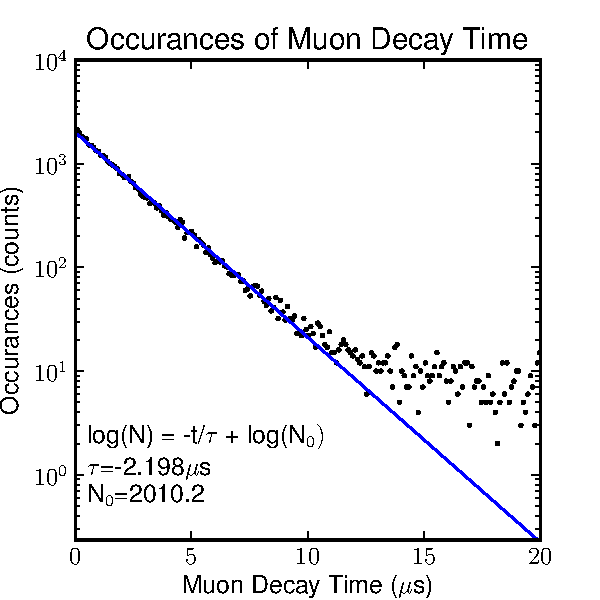
\includegraphics[width=3in]{images/fit1-eps-converted-to}
	\caption{Histogram with fit equation}
\end{figure}

\begin{figure}[h!]
	\centering
	\label{fig:fit1}
	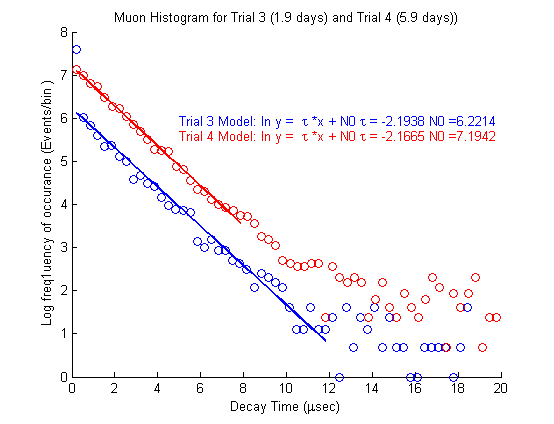
\includegraphics[width=3in]{images/hist1}
	\caption{Histogram Trial 1 and 2 with fit equation}
\end{figure}
\begin{figure}[h!]
	\centering
	\label{fig:fit1}
	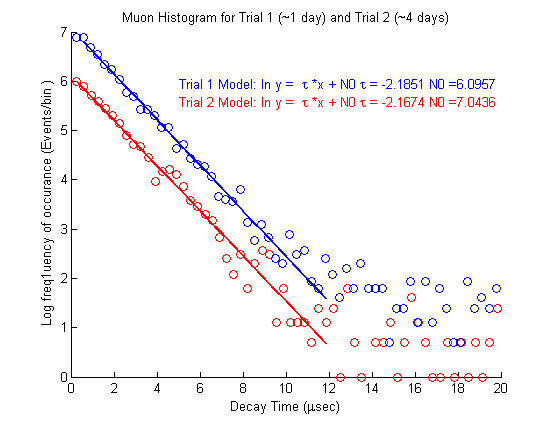
\includegraphics[width=3in]{images/hist2}
	\caption{Histogram Trial 3 and 4 with fit equation}
\end{figure}

\nocite{*}
\bibliography{references}
\bibliographystyle{plain}

\section{appendix}
\begin{figure}
	\centering
	\label{fig:table of values}
	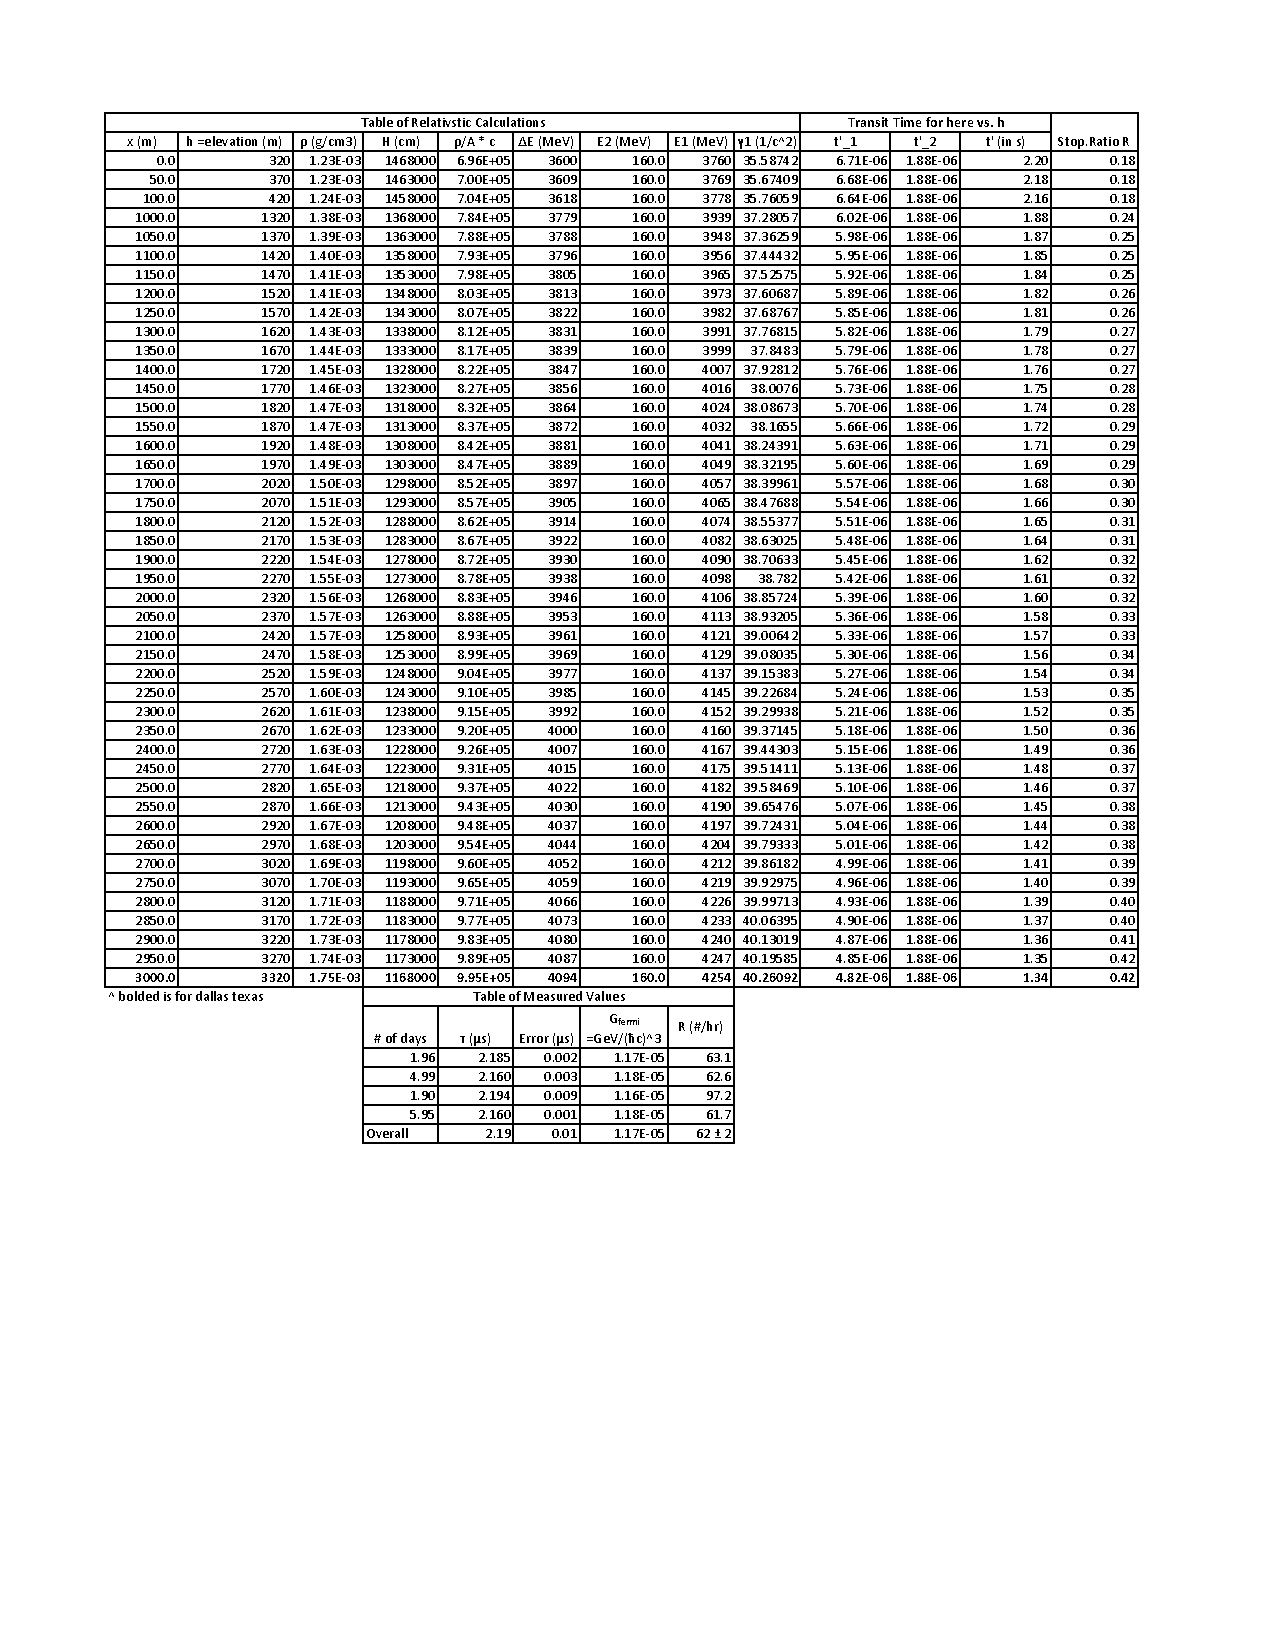
\includegraphics[width=6in]{images/Muon2}
	\caption{Table of Muon values}
\end{figure}
\end{document}

